\documentclass{exam}
\usepackage[utf8]{inputenc}
\usepackage[margin=1in]{geometry}
\usepackage{amsmath}
\usepackage{siunitx}
\usepackage{graphicx}
\usepackage{multicol}
\usepackage{etoolbox}
\usepackage{intcalc}
\usepackage{framed}
\usepackage{tabu}
\usepackage{tabularx}
\newcommand{\match}[2]{
	\begin{tabularx}{\textwidth}{r X}
		\fillin[#1][0.5 in] & #2
	\end{tabularx}}
\newcounter{wbcount}
\newcommand{\wbelem}[1]{\stepcounter{wbcount}
	\textbf{\Alph{wbcount}} & {#1}
	\ifnumequal{0}{\intcalcMod{\value{wbcount}}{\wbcolsize}}
		{\\}
		{&}
}
\newenvironment{wordbank}[1]{
	\renewcommand*{\arraystretch}{1.5} \def\wbcolsize{#1}
	\begin{center} \begin{framed}
	\begin{tabu} to \textwidth {*{#1}{X[1,l] X[5,l]}}
	}
	{\end{tabu} \end{framed} \end{center}
}
\setlength\answerclearance{3 pt}

\usepackage{xcolor}
\newcommand{\choiceblank}[1]{
	\ifprintanswers \underline{\ \ #1\ \ }
	\else \underline{\hspace{0.40 in}}
	\fi
	\vspace{0.05 in}
}
\newcommand{\fixcolspacing}{\vspace{0pt plus 1filll}\mbox{}}
\renewcommand{\solutiontitle}{}
\unframedsolutions
\SolutionEmphasis{\color{violet}}


\pagestyle{head}
\header{UT Invitational, Fall 2018}{Astronomy C - Page \thepage}{Team Number:\kern .5 in}
\headrule

\begin{document}
\begin{coverpages}
	\begin{center}
		\vspace{0.05 in}
		\par\noindent\textbf{\large  UT Invitational, Fall 2018}
		\vspace{0.05 in}
		\vspace{0.10 in}
		\par\noindent\textbf{\Huge   Astronomy C}
		\vspace{0.25 in}
		\par\noindent
		\vspace{0.05 in}
		\par\noindent
				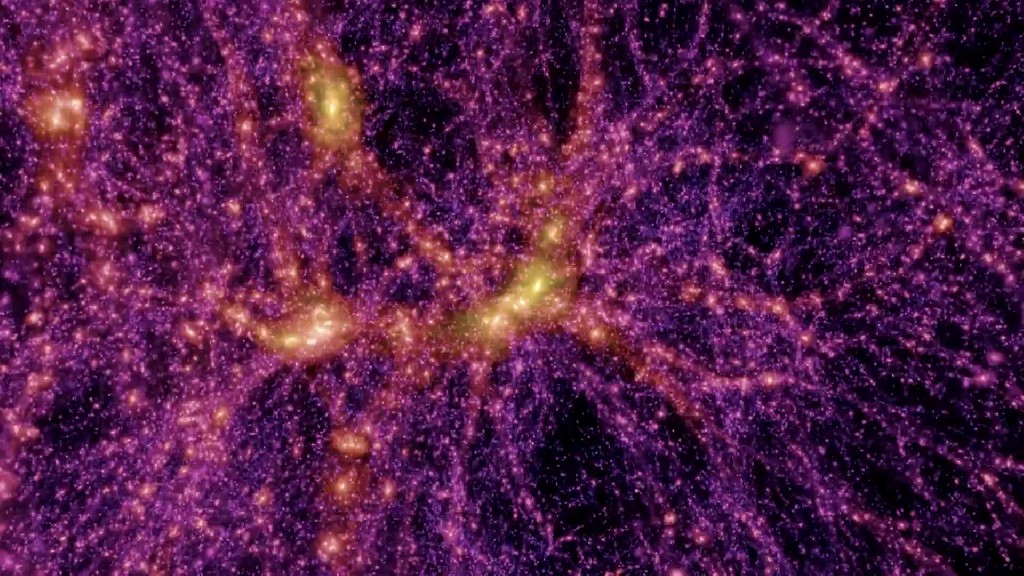
\includegraphics[width=.7\textwidth]{images/cover.jpg}
		\vspace{0.05 in}
		\vspace{0.25 in}
		\vspace{0.10 in}
		\vspace{0.15 in}
		\par
		\def\arraystretch{2}\tabcolsep=3pt
		\begin{tabular}{r r}
			\textbf{Competitors:} & \makebox[4in]{\hrulefill} \\
			\textbf{School Name:} & \makebox[4in]{\hrulefill} \\
			\textbf{Team Number:} & \makebox[4in]{\hrulefill} \\
		\end{tabular}
		\vspace{0.15 in}
	\end{center}
		\vspace{0.10 in}
	\par\noindent This test contains 4 sections; questions roughly increase in difficulty as the test progresses. If you're new to astronomy or Science Olympiad in general, welcome! The first parts of the test are hopefully accessible to you. For the dedicated veterans, I hope you'll find more challenging material near the end.
	\par As a result of this attempt to include questions from a wide distribution of difficulty, this test is long. You're not expected to finish the exam. You can complete the questions in the order that best suits your team's strengths.
	\par As always, you’ll have 50 minutes to complete the test. You may separate the pages; be sure to put your team number at the top of every page. Don’t feel obligated to write in complete sentences; your priority is to get all your ideas on paper quickly. Don't worry about keeping track of significant digits; one or two sigfigs is fine\footnote{As my professor puts it, ``Don't worry about numbers. They're not important.''}. No wifi allowed, don't cheat, etc. Tiebreaker: first question missed.
	\par Good Luck, Have Fun! And always remember: The Eyes of Texas Are Upon You!
		\vspace{0.10 in}
	\begin{center}
		\vspace{0.05 in}
		\par
		\def\arraystretch{2}\tabcolsep=3pt
		\begin{tabular}{r r}
			\textbf{{Written by:}}
			 & \textbf{Dhruva Karkada}, \textit{ dkarkada@gmail.com} \\
			 & \textbf{Aditya Shah}, \textit{ adityashah108@gmail.com} \\
		\end{tabular}
		\vspace{0.05 in}
	\end{center}
\end{coverpages}

\newpage
\par\noindent \textbf{\large  Part I: Matching}
	\par\noindent  2 points each. Each choice will be used exactly once.
\begin{wordbank}{3}
	\wbelem{47 Tucanae/X9}
	\wbelem{Abell 400}
	\wbelem{Antennae Galaxies}
	\wbelem{Cen A}
	\wbelem{Chandra deep field-south}
	\wbelem{ESO 137-001}
	\wbelem{IC 10}
	\wbelem{M100}
	\wbelem{M51}
	\wbelem{M81}
	\wbelem{NGC 4993}
	\wbelem{Phoenix Cluster}
	\wbelem{SN2014J}
	\wbelem{SPT 0346-52}
	\wbelem{Sagittarius A*}
\end{wordbank}
\begin{questions}
\setcounter{question}{0}
	\question\match{G}{The only starburst galaxy in the local group, containing about 110 observable X-ray sources.}
	\question\match{O}{The closest supermassive black hole to earth.}
	\question\match{D}{A bright radio galaxy, about 12 million lightyears away, with a strange ``dust lane'' feature.}
	\question\match{F}{A galaxy whose rapid velocity results in its gas being stripped off.}
	\question\match{I}{The Deep Sky Object (DSO) pictured in Image 1.}
	\question\match{N}{The farthest object in the DSO list.}
	\question\match{C}{The DSO pictured in Image 2.}
	\question\match{K}{The galaxy which hosted the first-detected gravitational wave event of neutron stars merging.}
	\question\match{A}{A white dwarf-black hole binary with orbital period 25 minutes.}
	\question\match{B}{A galaxy cluster containing two supermassive black holes doomed to merge in a few million years.}
	\question\match{E}{The deepest X-ray image ever taken.}
	\question\match{L}{A galaxy cluster containing a giant central galaxy with extreme starburst.}
	\question\match{M}{The DSO being pointed to in Image 3.}
	\question\match{H}{A grand design galaxy about 55 million lightyears away, with starburst concentrated in an inner ring.}
	\question\match{J}{A galaxy whose interactions with the Cigar galaxy is prompting starburst in the latter.}
\end{questions}

\newpage
\par\noindent \textbf{\large  Part II: Multiple Choice}
	\par\noindent  2 points each.
\setlength{\columnsep}{0.40 in}
\begin{multicols*}{2}
\renewcommand{\choiceshook}{\setlength{\leftmargin}{0.40 in}}
\renewcommand{\questionshook}{\setlength{\leftmargin}{0.0 in}}
\begin{questions}
\setcounter{question}{15}
	\question Which of the following lists the order of the main spectral types from hottest to coolest?
	\begin{choices}
		\CorrectChoice OBAFGKM
		\choice BOGAFMK
		\choice BOAGFKM
		\choice OBAGFMK
	\end{choices}
	\question Which of the following processes is responsible for preventing the sun from collapsing under its own weight?
	\begin{choices}
		\choice Nuclear fission
		\CorrectChoice Nuclear fusion
		\choice Solar beta reduction
		\choice Neutrino emission
	\end{choices}
	\question What are the three common stellar remnants?
	\begin{choices}
		\choice Red giant, planetary nebula, white dwarf
		\CorrectChoice White dwarf, neutron star, black hole
		\choice White dwarf, brown dwarf, red dwarf
		\choice Nebula, interstellar gas, white dwarf
	\end{choices}
	\question The spectral class of the sun is:
	\begin{choices}
		\choice A
		\choice F
		\CorrectChoice G
		\choice M
	\end{choices}
	\question Observe Image 4. Which letter denotes where the sun is located?
	\begin{choices}
		\choice A
		\CorrectChoice B
		\choice C
		\choice D
	\end{choices}
	\question Observe Image 4. Which letter denotes the location of Sag A*?
	\begin{choices}
		\choice A
		\choice B
		\CorrectChoice C
		\choice D
	\end{choices}
	\vfill\null\columnbreak
	\question Observe Image 4. Suppose a 1 solar mass star is located at point E. Which is the most likely fate for the star?
	\begin{choices}
		\CorrectChoice Planetary nebula and white dwarf
		\choice Undergo supernova
		\choice Collide with another star
		\choice Fall into the supermassive black hole at the center of the galaxy
	\end{choices}
	\question Our solar system
	\begin{choices}
		\choice Is spiraling outwards from the center of our galaxy.
		\choice Is spiraling inwards towards the center of our galaxy.
		\choice Is falling directly towards the center of our galaxy.
		\CorrectChoice Orbits the center of the milky way at approximately the same distance.
	\end{choices}
	\question Stars form when
	\begin{choices}
		\choice Planets gain enough mass to start glowing.
		\choice A planetary nebula collapses onto a white dwarf.
		\CorrectChoice A cloud of cool gas collapses due to its own gravity.
		\choice Scientists have no idea how stars form.
	\end{choices}
	\question \_\_\_ dwarfs are stellar remnants; \_\_\_ dwarfs are substellar objects; \_\_\_ dwarfs are main sequence stars.
	\begin{choices}
		\CorrectChoice White; brown; red
		\choice White; red; brown
		\choice Red; white; brown
		\choice Red; brown; white
	\end{choices}
	\question A star’s temperature
	\begin{choices}
		\CorrectChoice Increases towards the center.
		\choice Decreases towards the center.
		\choice Is fairly constant throughout the star.
		\choice Increases towards the center, until the deep core which is relatively cool.
	\end{choices}
	\question A very massive main-sequence star is likely to be
	\begin{choices}
		\CorrectChoice Very hot.
		\choice Very cool.
		\choice Larger than a red giant.
		\choice Smaller than a red dwarf.
	\end{choices}
	\vfill\null\columnbreak
	\question Imagine two stars orbiting each other. If the distance between them decreases, then the speed at which they orbit each other
	\begin{choices}
		\choice Decreases.
		\CorrectChoice Increases.
		\choice Is unchanged.
		\choice Not enough information
	\end{choices}
	\question About what percentage of main-sequence stars fuse hydrogen in their cores?
	\begin{choices}
		\choice 10\%
		\choice 40\%
		\choice 70\%
		\CorrectChoice 100\%
	\end{choices}
	\question Which of the following statements about black holes is FALSE?
	\begin{choices}
		\choice Their properties are described by Einstein’s theory of general relativity.
		\CorrectChoice It's impossible to orbit a black hole for a long period of time.
		\choice Time flows differently near a black hole.
		\choice Once something has fallen in, it can’t leave.
	\end{choices}
	\question Stars appear to twinkle because of
	\begin{choices}
		\choice Interfering nebulae between the star and earth.
		\choice Variations in their stellar atmospheres.
		\CorrectChoice Turbulence in earth’s atmosphere.
		\choice The brain’s inability to perceive point-sources of light.
	\end{choices}
	\question Evidence that the universe is expanding first came from
	\begin{choices}
		\choice Albert Einstein.
		\choice Annie Jump Cannon.
		\CorrectChoice Edwin Hubble.
		\choice Subrahmanyan Chandrasekhar.
	\end{choices}
	\question Light can be described\footnote{In this question we're ignoring quantum field theoretic formulations. If you don't know what that means, don't worry.} as
	\begin{choices}
		\choice Electromagnetic waves only.
		\choice Photons only.
		\CorrectChoice Either a particle or a wave depending on context.
		\choice Neither a particle nor a wave.
	\end{choices}
	\vfill\null\columnbreak
	\question Which of the following statements about the Big Bang model is FALSE?
	\begin{choices}
		\choice It asserts that the universe is 13.7 billion years old.
		\choice It suggests that the universe expanded from a singularity.
		\CorrectChoice It was the prevailing view of the universe during Newton’s time.
		\choice It replaced the idea that the universe is unchanging.
	\end{choices}
	\question The chemical makeup (by mass) of the universe is closest to:
	\begin{choices}
		\choice 31\% hydrogen, 25\% helium, 44\% other
		\choice 42\% hydrogen, 42\% helium, 16\% other
		\choice 53\% hydrogen, 43\% helium, 4\% other
		\CorrectChoice 73\% hydrogen, 25\% helium, 2\% other
	\end{choices}
	\question Supermassive black holes are
	\begin{choices}
		\choice Mostly found in very distant galaxies.
		\choice Concentrated at the center of the Milky Way.
		\choice Randomly distributed throughout the universe.
		\CorrectChoice Mostly found at the centers of galaxies.
	\end{choices}
	\question A star whose radius pulsates regularly is known as
	\begin{choices}
		\choice A blue supergiant.
		\choice A red giant.
		\CorrectChoice A Cepheid.
		\choice A pulsar.
	\end{choices}
	\question A pulsar is a special type of
	\begin{choices}
		\CorrectChoice Neutron star.
		\choice Brown dwarf.
		\choice Planetary nebula.
		\choice White dwarf.
	\end{choices}
	\question Since the universe is expanding, we notice that
	\begin{choices}
		\CorrectChoice Most galaxies seem to move away from us, with farther galaxies receding faster.
		\choice Most galaxies seem to move away from us, with equal recession rates.
		\choice Most galaxies are not moving relative to us, but the intergalactic dark energy is increasing.
		\choice Most galaxies are not moving relative to us, since universal expansion is a purely quantum phenomenon.
	\end{choices}
	\vfill\null\columnbreak
	\question Gravitational waves (which we can currently detect) can be produced by
	\begin{choices}
		\choice Rapidly rotating black holes.
		\CorrectChoice Black holes rapidly orbiting each other.
		\choice A supermassive black hole.
		\choice Any sufficiently dense object.
	\end{choices}
	\question The famous gravitational wave detection laboratory is called
	\begin{choices}
		\CorrectChoice LIGO.
		\choice Chandra.
		\choice APEX.
		\choice SETI.
	\end{choices}
	\question The brightness of blackbody radiation is limited by
	\begin{choices}
		\choice The photoionization limit.
		\choice The Chandrasekhar limit.
		\CorrectChoice The Eddington limit.
		\choice The Planck limit.
	\end{choices}
	\question If the Milky Way were the size of a frisbee, the nearest spiral galaxy would be
	\begin{choices}
		\choice A few inches away.
		\CorrectChoice Several feet away.
		\choice Hundreds of yards away.
		\choice A few miles away.
	\end{choices}
	\question Which of the following is NOT a galaxy in the local group?
	\begin{choices}
		\choice Andromeda Galaxy
		\CorrectChoice Whirlpool Galaxy
		\choice Large Magellanic Cloud
		\choice Triangulum Galaxy
	\end{choices}
	\question When two galaxies collide:
	\begin{choices}
		\choice The stars are totally unaffected.
		\CorrectChoice Some stars may be flung out, but most will not encounter star-star collisions.
		\choice Stars will not be flung out, but there will be many star-star collisions.
		\choice We have no way of knowing whether or how galaxies collide.
	\end{choices}
	\vfill\null\columnbreak
	\question Stars tend to form in galaxies because
	\begin{choices}
		\CorrectChoice Gas in intergalactic space is too sparse.
		\choice The magnetic force of the galactic nucleus is critical in star formation.
		\choice Most stars don’t form in galaxies, but the gravitational pull of galaxies results in stars eventually collecting in galaxies.
		\choice Most stars don’t form in galaxies; the extragalactic stars are just exceedingly dim.
	\end{choices}
	\question Which of the following is FALSE\footnote{Assume that Keplerian physics holds; we aren't concerned with the precision of general relativity.}?
	\begin{choices}
		\CorrectChoice The orbit of a planet is an ellipse, and the star is always at the center of the ellipse.
		\choice A small planet orbiting a star sweeps out equal areas in equal time intervals.
		\choice Stars orbiting each other obey Kepler’s 3rd law.
		\choice Planets orbiting a star obey Kepler’s laws.
	\end{choices}
	\question Wien’s displacement law gives us information about
	\begin{choices}
		\choice The intrinsic luminosities of Cepheid stars
		\choice The hydrogen ionization temperature of a star
		\choice The orbital velocities of stars in a galaxy
		\CorrectChoice The peak blackbody radiation wavelength of a star
	\end{choices}
	\question A starburst can be caused by all of the following except
	\begin{choices}
		\choice Interaction with another galaxy.
		\choice Sudden morphological changes in the galaxy.
		\CorrectChoice An active galactic nucleus.
		\choice Interaction with hot intergalactic dust.
	\end{choices}
	\question The balance between a star’s inward pull of gravity and its outwards pressure gradient is called
	\begin{choices}
		\choice Quasistatic stellar continuum.
		\choice Stellar equilibrium.
		\choice Stellar uniformity.
		\CorrectChoice Hydrostatic equilibrium.
	\end{choices}
\end{questions}
\end{multicols*}
\renewcommand{\choiceshook}{}
\renewcommand{\questionshook}{}

\newpage
\par\noindent \textbf{\large  Part III: Free Response}
	\par\noindent  Each sub-part is worth 3 points.
\begin{questions}
	\setcounter{question}{50}
	\question The Chandra observatory specializes in looking for x-ray sources.
	\begin{parts}
		\part X-rays are considered to be “energetic” compared to, for example, infrared radiation. Why is this?
		\part Many bright X-ray sources are thought to be binary systems containing black holes. How are the X-rays produced? Briefly explain the relevant physics.
		\part Why isn’t all the X-ray light sucked into the black hole?
	\end{parts}
	\question Given that cosmic background radiation (CMB) has a temperature of 2.7 Kelvin, at what wavelength is it the brightest, in meters?
	\question A star has a parallax angle of 0.0133 arcseconds when viewed from Earth. Over the past 5 years, its position in the sky has changed by 0.05 arcseconds.
	\begin{parts}
		\part How far away is this star from Earth, in parsecs?
		\part What is the proper motion of this star, in arcseconds per year?
		\part What is the star’s tangential velocity, in km/s?
		\part Radial velocity measurements show that the H$\alpha$ line is shifted from 656.28 nm to 656.30 nm. What is this star’s radial velocity, in km/s?
		\part Given your answers to parts (c) and (d), what is the true space velocity of this star, in km/s? Hint: think about using the Pythagorean Theorem.
		\part An astronomy student suggests using Hubble’s Law as means of checking the star’s distance (previously calculated in part (a)). What distance, in parsecs, does this student get when they carry out the calculation? Assume Hubble’s constant is 70 km/s/Mpc.
		\part Explain a cause of the discrepancy between the distances calculated in part (a) and part (f). Which distance is likely more accurate?
	\end{parts}
	\question The supermassive black hole at the center of a galaxy has a mass of $\num{4e6}$ solar masses. A star is travelling around it in a very elliptical orbit. Because the supermassive black hole is far more massive than the star, assume the star’s mass is negligible.
	\begin{parts}
		\part Long term observations of the star show that it has an orbital period of 22 years. What is its semimajor axis, in AU?
		\part At its periapsis (closest point in the orbit), the star’s distance from the supermassive black hole is one-half of its semimajor axis. At this point, how fast is the star moving, in m/s?
		\part The apoapsis (furthest point in the orbit) of this star’s path is three times its periapsis. What is the eccentricity of its orbit?
	\end{parts}
	\question Examine Images 5, 6, and 7. These are observations of the same object, in 3 different bands: blue, red, and far ultraviolet respectively.
	\begin{parts}
		\part What is pictured? Be as specific as possible.
		\part All the images feature a dark band, which is highlighted in red. What is most likely causing the dark band?
		\part Image 7 looks different than the other two. What is causing the far-UV glow in the upper and lower regions?
	\end{parts}
\end{questions}

\newpage
\par\noindent \textbf{\large  Part IV: Research Literacy}
	\par\noindent  Each question is worth 3 points.
		\vspace{0.10 in}
	\par\noindent \noindent The following excerpt is from the abstract of a May 2018 research paper (co-authored by a researcher here at UT!) published in the research journal \textit{The Astrophysical Journal}.
		\vspace{0.10 in}
	\par \noindent\textbf{GW170817 Most Likely Made a Black Hole}
	\par There are two outstanding issues regarding the neutron-star merger event GW170817: the nature of the compact remnant and the interstellar shock. The mass of the remnant of GW170817, $\approx 2.7 M_\odot$, implies the remnant could be either a massive, rotating, neutron star, or a black hole. We report Chandra [...] observations made in 2017 December and 2018 January, and we reanalyze earlier observations from 2017 August and 2017 September, in order to address these unresolved issues. We estimate the X-ray flux from a neutron star remnant and compare that to the measured X-ray flux. If we assume that the spin-down luminosity of any putative neutron star is converted to pulsar wind nebula X-ray emission in the $0.5-8$ keV band with an efficiency of $10^{-3}$, for a dipole magnetic field with $3\times 10^{11} \;\mathrm{G} < B < 10^{14} \;\mathrm{G}$, a rising X-ray signal would result and would be brighter than that observed by day 107; we therefore conclude that the remnant of GW170817 is most likely a black hole. Independent of any assumptions of X-ray efficiency, however, if the remnant is a rapidly-rotating, magnetized, neutron star, the total energy in the external shock should rise by a factor $\approx 10^2$ [...] after a few years; therefore, Chandra observations over the next year or two that do not show substantial brightening will rule out such a remnant. The same observations can distinguish between two different models for the relativistic outflow, either an angular or radially varying structure.
\begin{questions}
	\setcounter{question}{55}
	\question Briefly summarize (1-2 sentences) the researchers' strategy to show that the remnant is probably not a neutron star.
	\question The researchers claim that since the remnant's mass is $\approx 2.7 M_\odot$, it ``could be either a massive, rotating, neutron star, or a black hole.'' If the object were a neutron star, why do the scientists conclude it must be rotating?
	\question What is the ``spin-down luminosity''? Briefly explain the mechanism.
	\question Why would a neutron star remnant display brightening over the next few years?
	\question What might the ``relativistic outflow'' be referring to?
\end{questions}
	\par\noindent \hrule
		\vspace{0.10 in}
	\par \noindent Image 8, from Larson and Tinsley (1978), shows $U-B$ vs. $B-V$ color for “normal morphology” galaxies from the Hubble Atlas (left) and for “peculiar” galaxies from the Arp Atlas (right). The red letters have been added in by the authors of this test to denote locations on the diagram. Notice how the “peculiar” galaxies have significantly more scatter in their color.
\begin{questions}
	\setcounter{question}{60}
	\question What do “$U-B$” and “$B-V$” mean?
	\question Which location (A-D) represents the “bluest” galaxy? Disregard whether that galaxy exists and simply go by the letter’s location on the diagram.
	\question The two open circles in the diagram for “peculiar” galaxies from the Arp Atlas are Type 1 Seyfert galaxies. What is the difference between the spectra of Type 1 and Type 2 Seyfert Galaxies?
\end{questions}
	\par\noindent \noindent Image 9 shows $U-B$ vs. $B-V$ for galaxies from the Arp Atlas, separated into non-interacting (left) and interacting (right).
\begin{questions}
	\setcounter{question}{63}
	\question Based on this diagram, what seems to be the cause of the “peculiar” galaxies’ greater variation in color?
	\question “Peculiar” galaxies are often sites of short, yet intense bursts of star formation. Explain how galaxy interactions could lead to these bursts.
\end{questions}

\newpage
\par\noindent \textbf{\large  Images}
		\par\noindent
	\begin{center}
		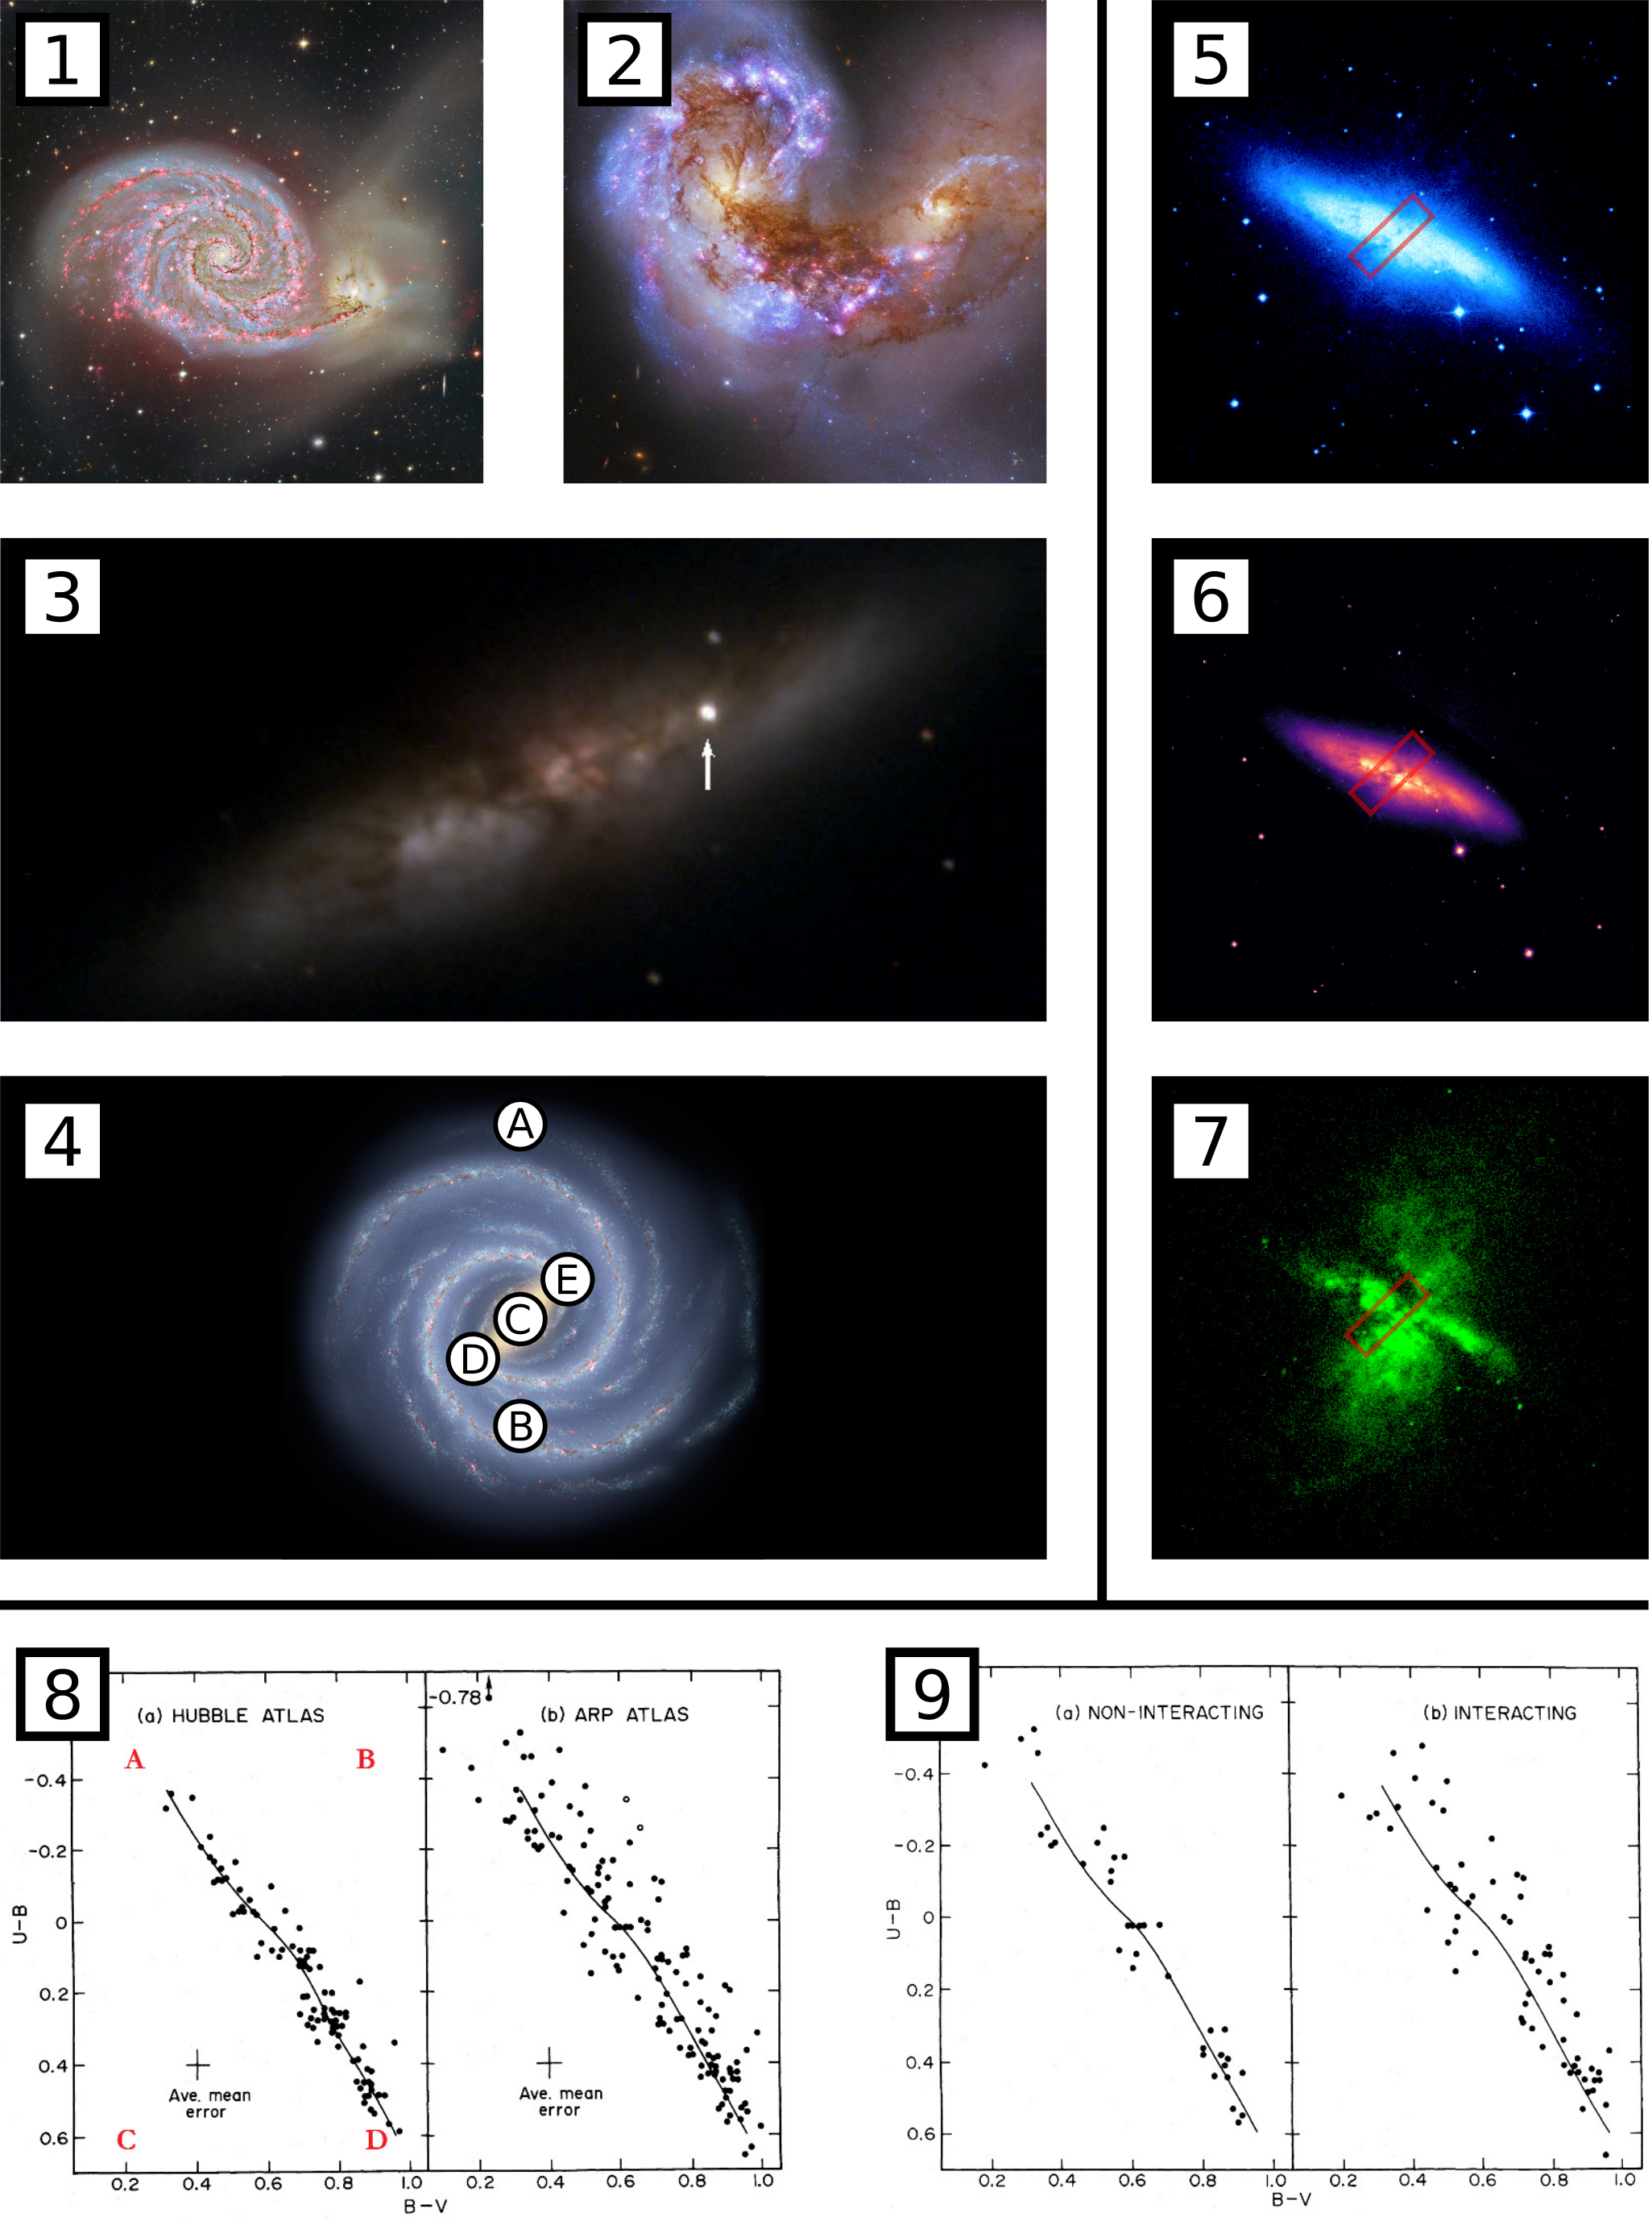
\includegraphics[width=.9\textwidth]{images/diagram-sheet.png}
	\end{center}
\newpage
\section*{Answer Sheet}
	\raggedcolumns
	\begin{multicols}{5}
	\begin{enumerate}
	\setcounter{enumi}{0}
	\item \choiceblank{G}
	\item \choiceblank{O}
	\item \choiceblank{D}
	\item \choiceblank{F}
	\item \choiceblank{I}
	\item \choiceblank{N}
	\item \choiceblank{C}
	\item \choiceblank{K}
	\item \choiceblank{A}
	\item \choiceblank{B}
	\item \choiceblank{E}
	\item \choiceblank{L}
	\item \choiceblank{M}
	\item \choiceblank{H}
	\item \choiceblank{J}
	\end{enumerate}
	\end{multicols}
	\raggedcolumns
	\begin{multicols}{5}
	\begin{enumerate}
	\setcounter{enumi}{15}
	\item \choiceblank{A}
	\item \choiceblank{B}
	\item \choiceblank{B}
	\item \choiceblank{C}
	\item \choiceblank{B}
	\item \choiceblank{C}
	\item \choiceblank{A}
	\item \choiceblank{D}
	\item \choiceblank{C}
	\item \choiceblank{A}
	\item \choiceblank{A}
	\item \choiceblank{A}
	\item \choiceblank{B}
	\item \choiceblank{D}
	\item \choiceblank{B}
	\item \choiceblank{C}
	\item \choiceblank{C}
	\item \choiceblank{C}
	\item \choiceblank{C}
	\item \choiceblank{D}
	\item \choiceblank{D}
	\item \choiceblank{C}
	\item \choiceblank{A}
	\item \choiceblank{A}
	\item \choiceblank{B}
	\item \choiceblank{A}
	\item \choiceblank{C}
	\item \choiceblank{B}
	\item \choiceblank{B}
	\item \choiceblank{B}
	\item \choiceblank{A}
	\item \choiceblank{A}
	\item \choiceblank{D}
	\item \choiceblank{C}
	\item \choiceblank{D}
	\end{enumerate}
	\end{multicols}
	\begin{questions}
	\setcounter{question}{50}
	\question
		\begin{parts}
		\part
			\ \vspace{36 pt}
		\part
			\ \vspace{52 pt}
		\part
			\ \vspace{36 pt}
		\end{parts}
	\question
		\ \vspace{36 pt}
	\question
		\begin{parts}
		\part
			\ \vspace{36 pt}
		\part
			\ \vspace{36 pt}
		\part
			\ \vspace{20 pt}
		\part
			\ \vspace{36 pt}
		\part
			\ \vspace{20 pt}
		\part
			\ \vspace{20 pt}
		\part
			\ \vspace{68 pt}
		\end{parts}
	\question
		\begin{parts}
		\part
			\ \vspace{36 pt}
		\part
			\ \vspace{52 pt}
		\part
			\ \vspace{20 pt}
		\end{parts}
	\question
		\begin{parts}
		\part
			\ \vspace{4 pt}
		\part
			\ \vspace{20 pt}
		\part
			\ \vspace{20 pt}
		\end{parts}
	\end{questions}
	\begin{questions}
	\setcounter{question}{55}
	\question
		\ \vspace{36 pt}
	\question
		\ \vspace{52 pt}
	\question
		\ \vspace{36 pt}
	\question
		\ \vspace{36 pt}
	\question
		\ \vspace{4 pt}
	\end{questions}
	\begin{questions}
	\setcounter{question}{60}
	\question
		\ \vspace{20 pt}
	\question
		\ \vspace{4 pt}
	\question
		\ \vspace{36 pt}
	\end{questions}
	\begin{questions}
	\setcounter{question}{63}
	\question
		\ \vspace{20 pt}
	\question
		\ \vspace{36 pt}
	\end{questions}
\end{document}